\documentclass{beamer}

\usepackage[utf8]{inputenc}
\usepackage[T1]{fontenc}
\usepackage{graphicx}
\usepackage{hyperref}

\title{Challenge IA : Présentation finale}
\author{Groupe : Couture Vision}
\institute{Membres : Noémie GUISNEL, Pierre JOURDIN, Clément FLORVAL, \\ Louis GAUTHIER, Anthony QUENTIN}
\date{\today}

\setbeamertemplate{footline}{
  \leavevmode%
  \hbox{%
  \begin{beamercolorbox}[wd=.5\paperwidth,ht=2.25ex,dp=1ex,center]{author in head/foot}%
    \usebeamerfont{author in head/foot}\insertshortauthor
  \end{beamercolorbox}%
  \begin{beamercolorbox}[wd=.5\paperwidth,ht=2.25ex,dp=1ex,right]{date in head/foot}%
    \insertframenumber{} / \inserttotalframenumber\hspace*{2ex}
  \end{beamercolorbox}}%
  \vskip0pt%
}

\begin{document}

\frame{\titlepage}

\begin{frame}{Sommaire}
\tableofcontents
\end{frame}

\section{Jeu de données}
\begin{frame}{Jeu de données}
\begin{columns}
    \column{0.5\textwidth}
    \begin{figure}
        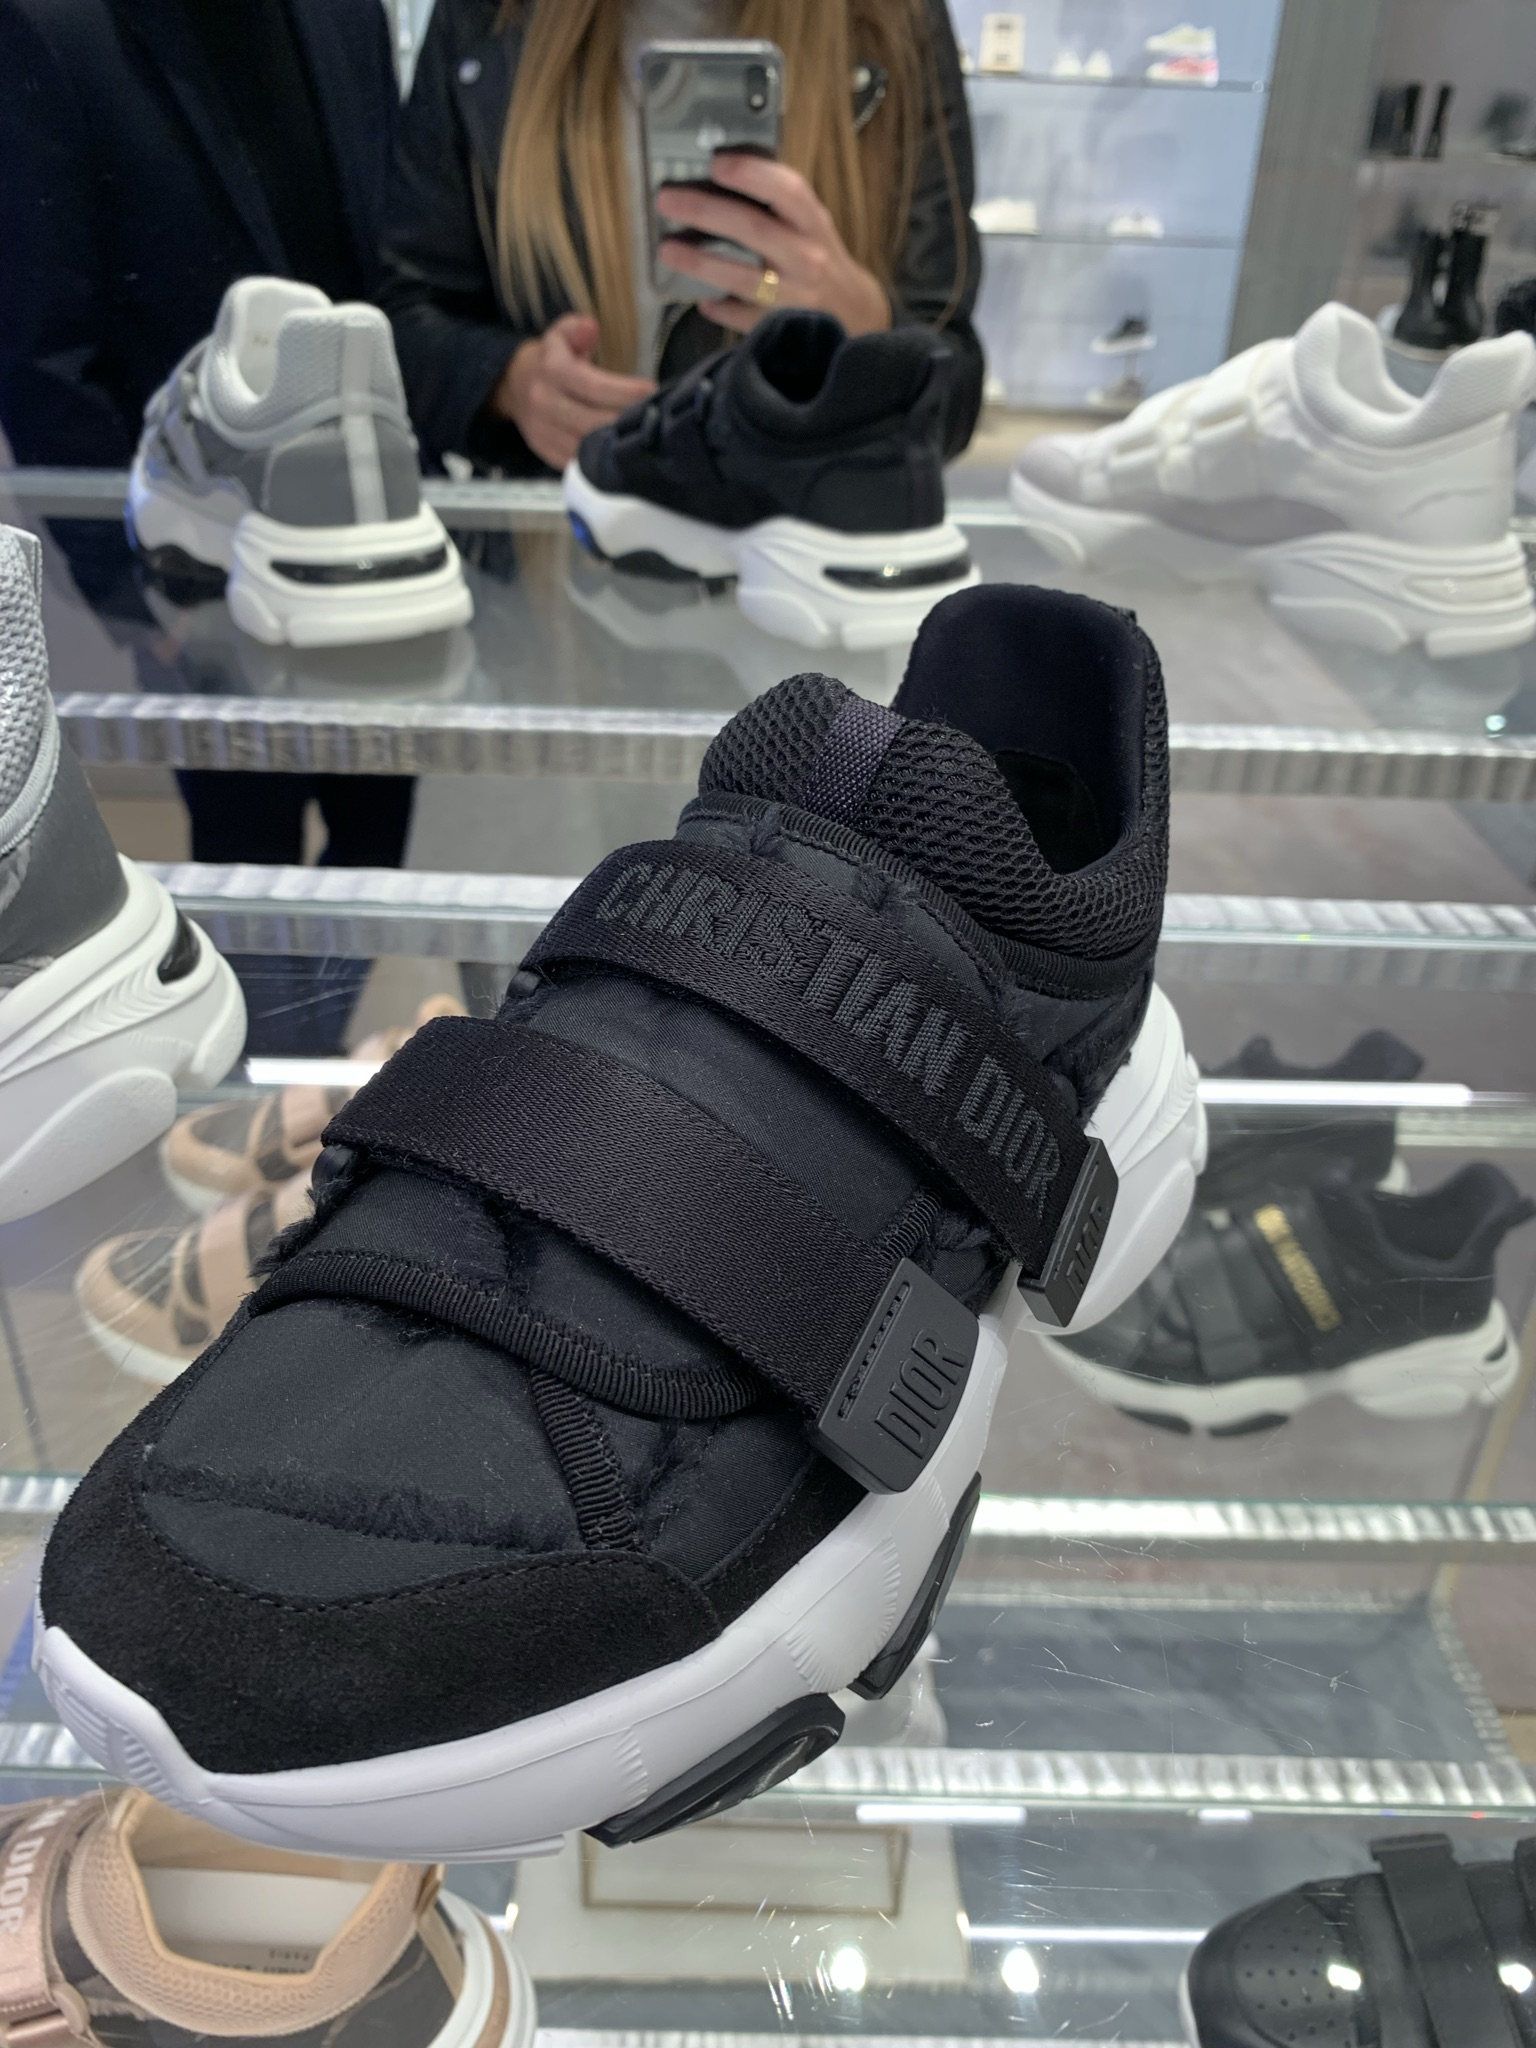
\includegraphics[width=0.6\textwidth]{assets/shoe_test.jpg}
        \caption{Image de test}
    \end{figure}
    \column{0.5\textwidth}
    \begin{figure}
        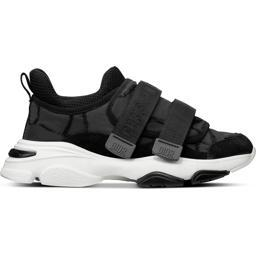
\includegraphics[width=0.6\textwidth]{assets/shoe_reference.jpeg}
        \caption{Image DAM}
    \end{figure}
\end{columns}
\vspace{0.5cm}
\begin{block}{Objectif}
\begin{itemize}
    \item Pour une image test d'article, trouver l'article (donc la référence) correspondant dans la base DAM (2766 articles).
    \item L'article doit être parmi les 1, 3 ou 5 références proposées.
\end{itemize}
\end{block}
\end{frame}

\begin{frame}{Jeu de données : Difficultés}
\begin{itemize}
    \item Grand nombre d'articles dans la base DAM (2766 articles).
    \item Unique photo par classe : difficile de faire de la classification
    \item Les images (surtout celles du test) ne sont pas standardisées (background, orientation...)
    \item Images très similaires dans DAM.
    \item Deux images de test dont le label n'est pas présent dans DAM.
\end{itemize}
\end{frame}


\section{Intuitions}
\begin{frame}{Intuitions}
\begin{itemize}
    \item Utilisation d'un modèle permettant d'extraire l'article de l'image et de mettre un fond blanc derrière.
    \item Utilisation d'un modèle pré-entraîné pour créer des embeddings sur les images DAM et les images de test.
    \item Pour chaque image de test, calcul des similarités cosinus avec tous les embeddings des images DAM et affichage des 5 meilleures similarités (Top-5).
\end{itemize}
\end{frame}

\begin{frame}{Modèles utilisés}
    \begin{itemize}
        \item \textbf{Extraction et traitement de l'article} : Utilisation de \texttt{RMBG-2.0} pour rogner l'image et supprimer le fond. 
        \item \textbf{Embeddings d'image} : Modèle ViT par Google (Base Patch-32, 86.4M paramètres).
        \item \textbf{Triplet Network} : Permet d'optimiser les embeddings pour réduire la distance cosinus entre des images similaires.
    \end{itemize}
    \end{frame}

\section{Principe et architecture du modèle retenu}
\begin{frame}{Traitement des images}
    \footnotesize
    \textbf{Suppression du fond avec \texttt{rembg} et recentrage de l'objet}
    \begin{itemize}
        \item Les images à inférer contiennent un arrière-plan indésirable.
        \item Utilisation de la bibliothèque \texttt{rembg} avec le modèle \texttt{u2net} pour retirer le fond. Objectif : réduire le bruit pour l'extraction des caractéristiques. 
        \item Ensuite, un traitement d’image identifie les pixels non transparents pour \textbf{recentrer et recadrer} l’objet.
    \end{itemize}
    \begin{columns}
        \column{0.5\textwidth}
        \begin{figure}
            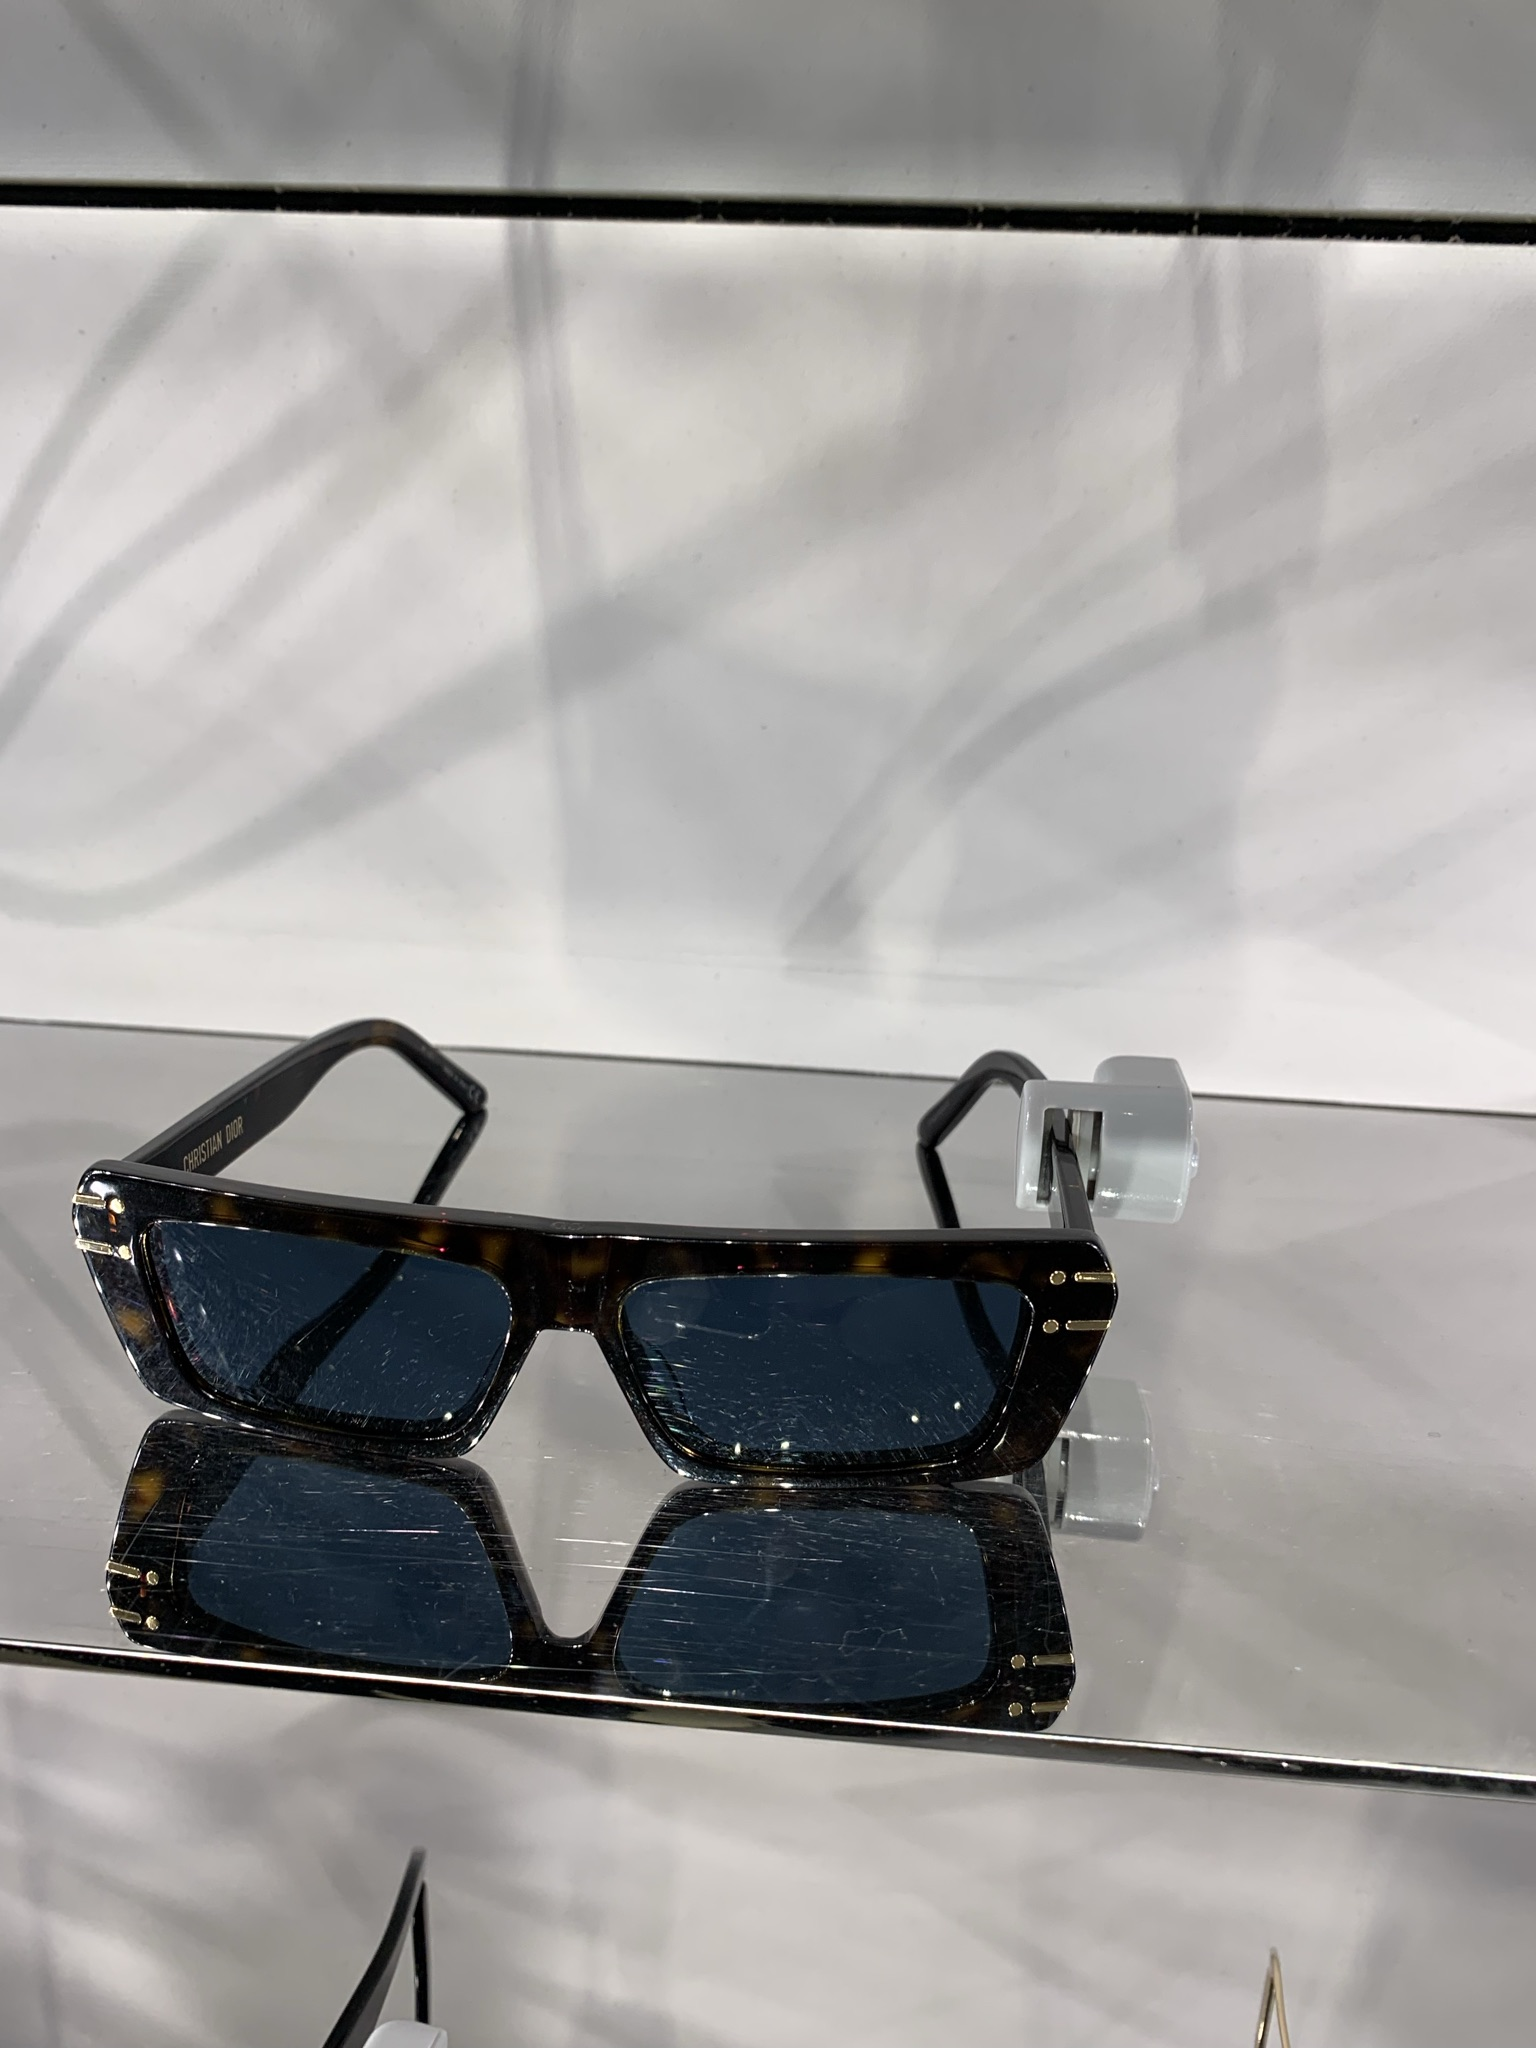
\includegraphics[width=0.4\textwidth]{assets/IMG_6883.jpg}
            \caption{Example of Image test}
        \end{figure}
        \column{0.5\textwidth}
        \begin{figure}
            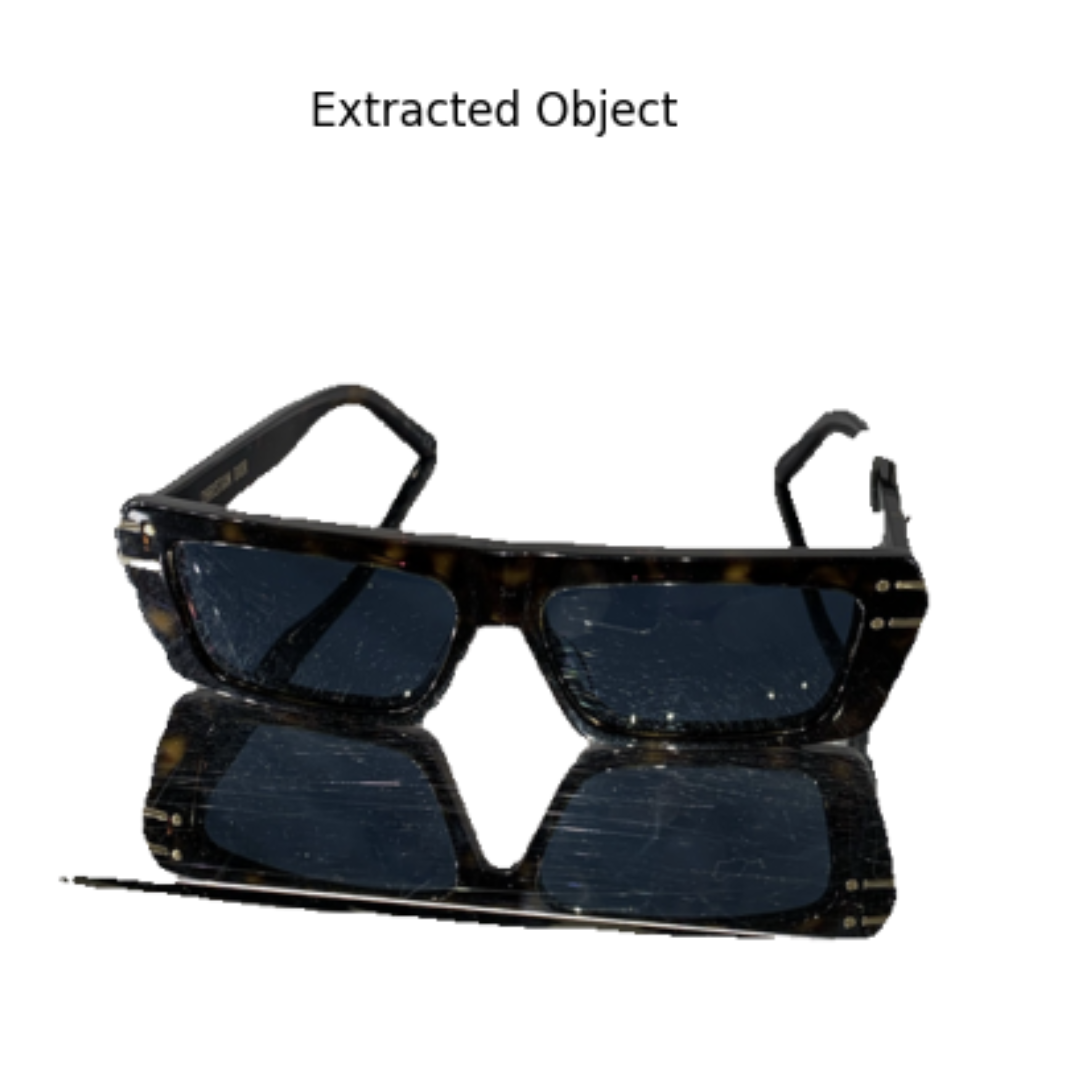
\includegraphics[width=0.4\textwidth]{assets/glasses_rembg.png}
            \caption{Extracted object with rembg}
        \end{figure}
    \end{columns}
\end{frame}

\begin{frame}{Amélioration avec \texttt{RMBG-2.0}}
    \footnotesize
    \textbf{Utilisation du modèle \texttt{briaai/RMBG-2.0} pour une meilleure suppression du fond}
    \begin{itemize}
        \item Le modèle précédent pouvait générer des artefacts ou des découpages imprécis.
        \item Amélioration de la qualité du traitement en utilisant le modèle \texttt{briaai/RMBG-2.0}.
        \item Ce modèle utilise des techniques avancées pour un détourage plus précis et net.
    \end{itemize}
    \begin{columns}
        \column{0.5\textwidth}
        \begin{figure}
            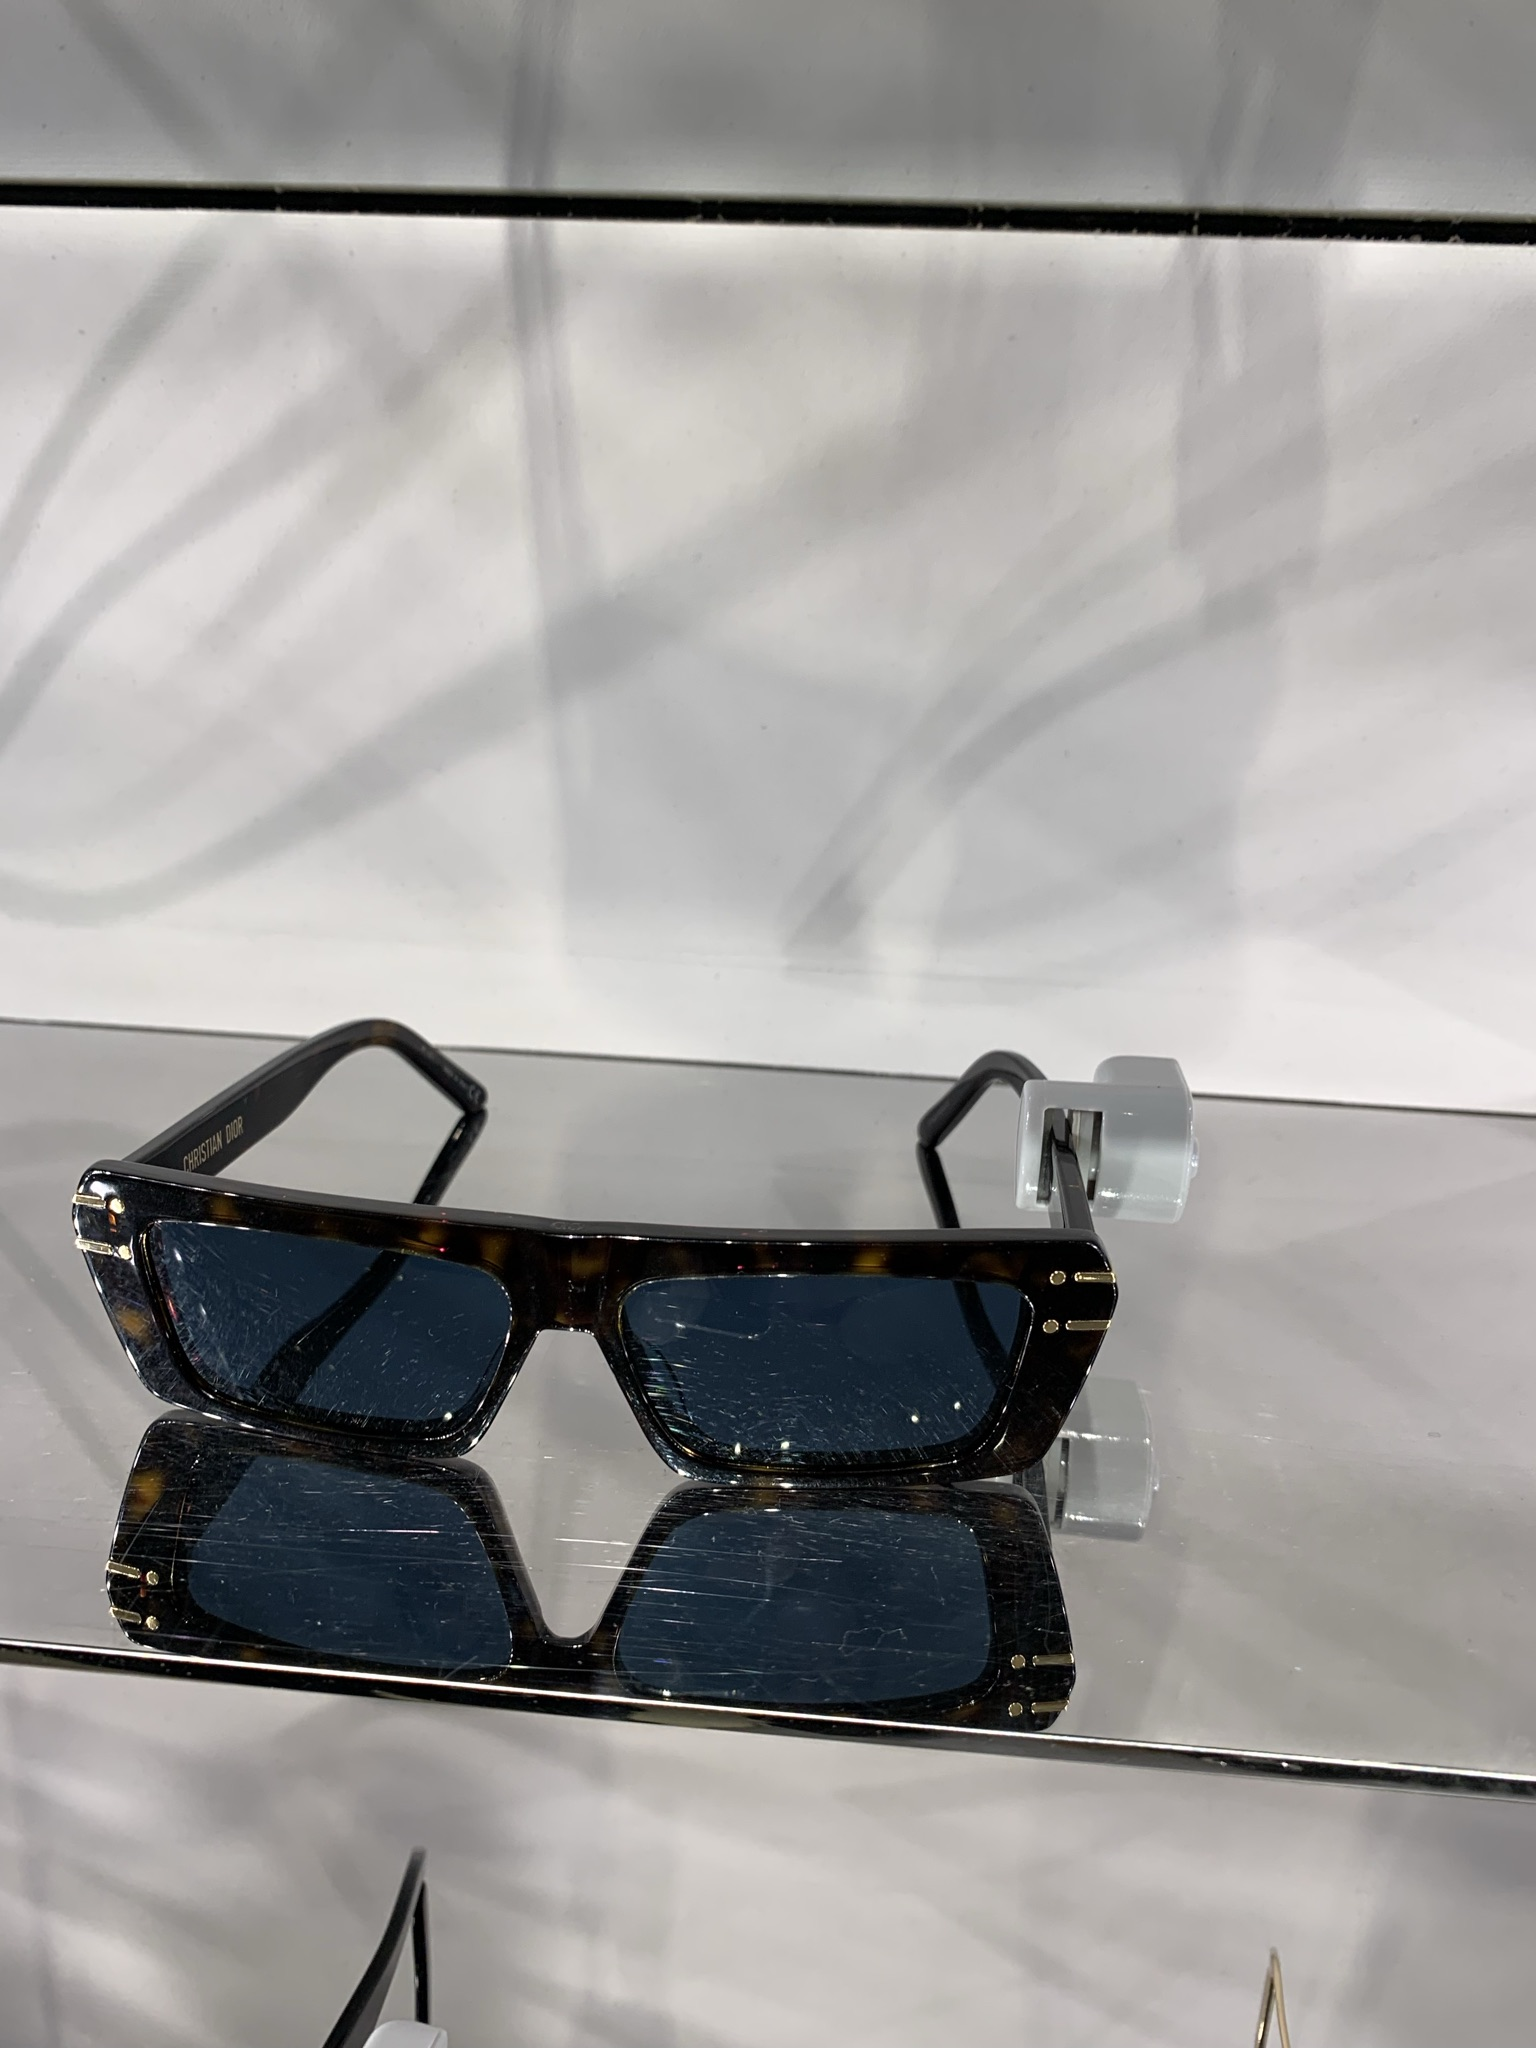
\includegraphics[width=0.4\textwidth]{assets/IMG_6883.jpg}
            \caption{Example of Image test}
        \end{figure}
        \column{0.6\textwidth}
        \begin{figure}
            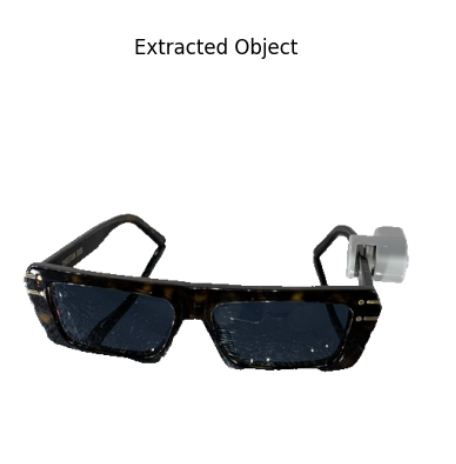
\includegraphics[width=0.4\textwidth]{assets/glasses_rmbg_2.png}
            \caption{Extracted object with rmbg-2.0}
        \end{figure}
    \end{columns}
\end{frame}

\begin{frame}{Comparaison des méthodes de suppression de fond}
    \textbf{Tableau comparatif des performances techniques}
    \begin{table}[]
        \centering
        \resizebox{\textwidth}{!}{
        \begin{tabular}{|l|c|c|}
            \hline
            \textbf{Critère} & \textbf{U2Net (rembg)} & \textbf{RMBG-2.0} \\
            \hline
            Architecture du modèle & U-Net modifié & développé à partir de BiRefNet \\
            \hline
            Nombre de paramètres & 44M & 221M \\
            \hline
            Qualité du détourage & Moyenne (bords flous) & Excellente (détails fins) \\
            \hline
            Rapidité de traitement & Rapide & Un peu plus lent \\
            \hline
            Consommation mémoire & Modérée & Plus élevée \\
            \hline
            Adaptabilité aux arrière-plans complexes & Moyenne & Très bonne \\
            \hline
        \end{tabular}
        }
        \caption{Comparaison entre U2Net et RMBG-2.0}
    \end{table}
    \begin{itemize}
        \item \textbf{RMBG-2.0 et recentrage de l'objet} sont appliqués aux images du DAM et à chaque image destinée à l'inférence
    \end{itemize}
\end{frame}

\begin{frame}{Présentation du Modèle ViT Base Patch32 224}
    \begin{itemize}
        \item \textbf{Nom du Modèle} : \texttt{google/vit-large-patch16-224}
        \item \textbf{Origine} : Développé par Google
        \item \textbf{Nombre de Paramètres} : Environ 86 millions
        \item \textbf{Pré-entraînement} : 
        \begin{itemize}
            \item Dataset : ImageNet
            \item Contenu : Environ 1.2 million d'images couvrant 1000 classes
        \end{itemize}
    \end{itemize}
    \vspace{0.5cm}
\end{frame}

\section{Amélioration des résultats}
\begin{frame}{Amélioration des résultats}
\begin{itemize}
    \item \textbf{Data augmentation} : Certaines images de test ne sont pas prises du même angle que les images DAM.
    \begin{itemize}
        \item Utilisation de \textbf{TRELLIS} pour générer des modèles 3D.
    \end{itemize}
    \item Recadrage et recentrage des images.
    \item Tests de nombreux modèles d'embedding: Microsoft ResNet-50, DinoV2, Nomic EmbedVision... les meilleurs résultats avec ViT de Google.
    \item Comparaison de différentes méthodes d'aggrégation des embeddings: mean, max, min, concaténation, CLS seulement... max donne les meilleurs résultats.
    \item Comparaison de différentes métriques de similarité: cosine et euclidean, cosine donne les meilleurs résultats.
\end{itemize}
\end{frame}


\begin{frame}{Data augmentation avec un modèle de géneration 3D}
    \begin{itemize}
        \item Nous avons utilisé \textbf{TRELLIS} pour générer 2700 modèles 3D des assets du DAM.
        \item 8 rendus \textbf{Blender} à des angles différents pour chaque modèle.
    \end{itemize}
    
    \begin{columns}
        \column{0.5\textwidth}
        \begin{figure}
            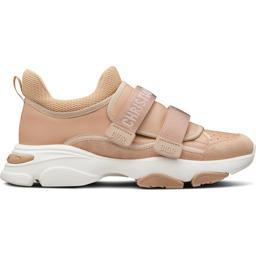
\includegraphics[width=0.65\textwidth]{assets/trellis_input.png}
            \caption{Input for TRELLIS}
        \end{figure}
        \column{0.5\textwidth}
        \begin{figure}
            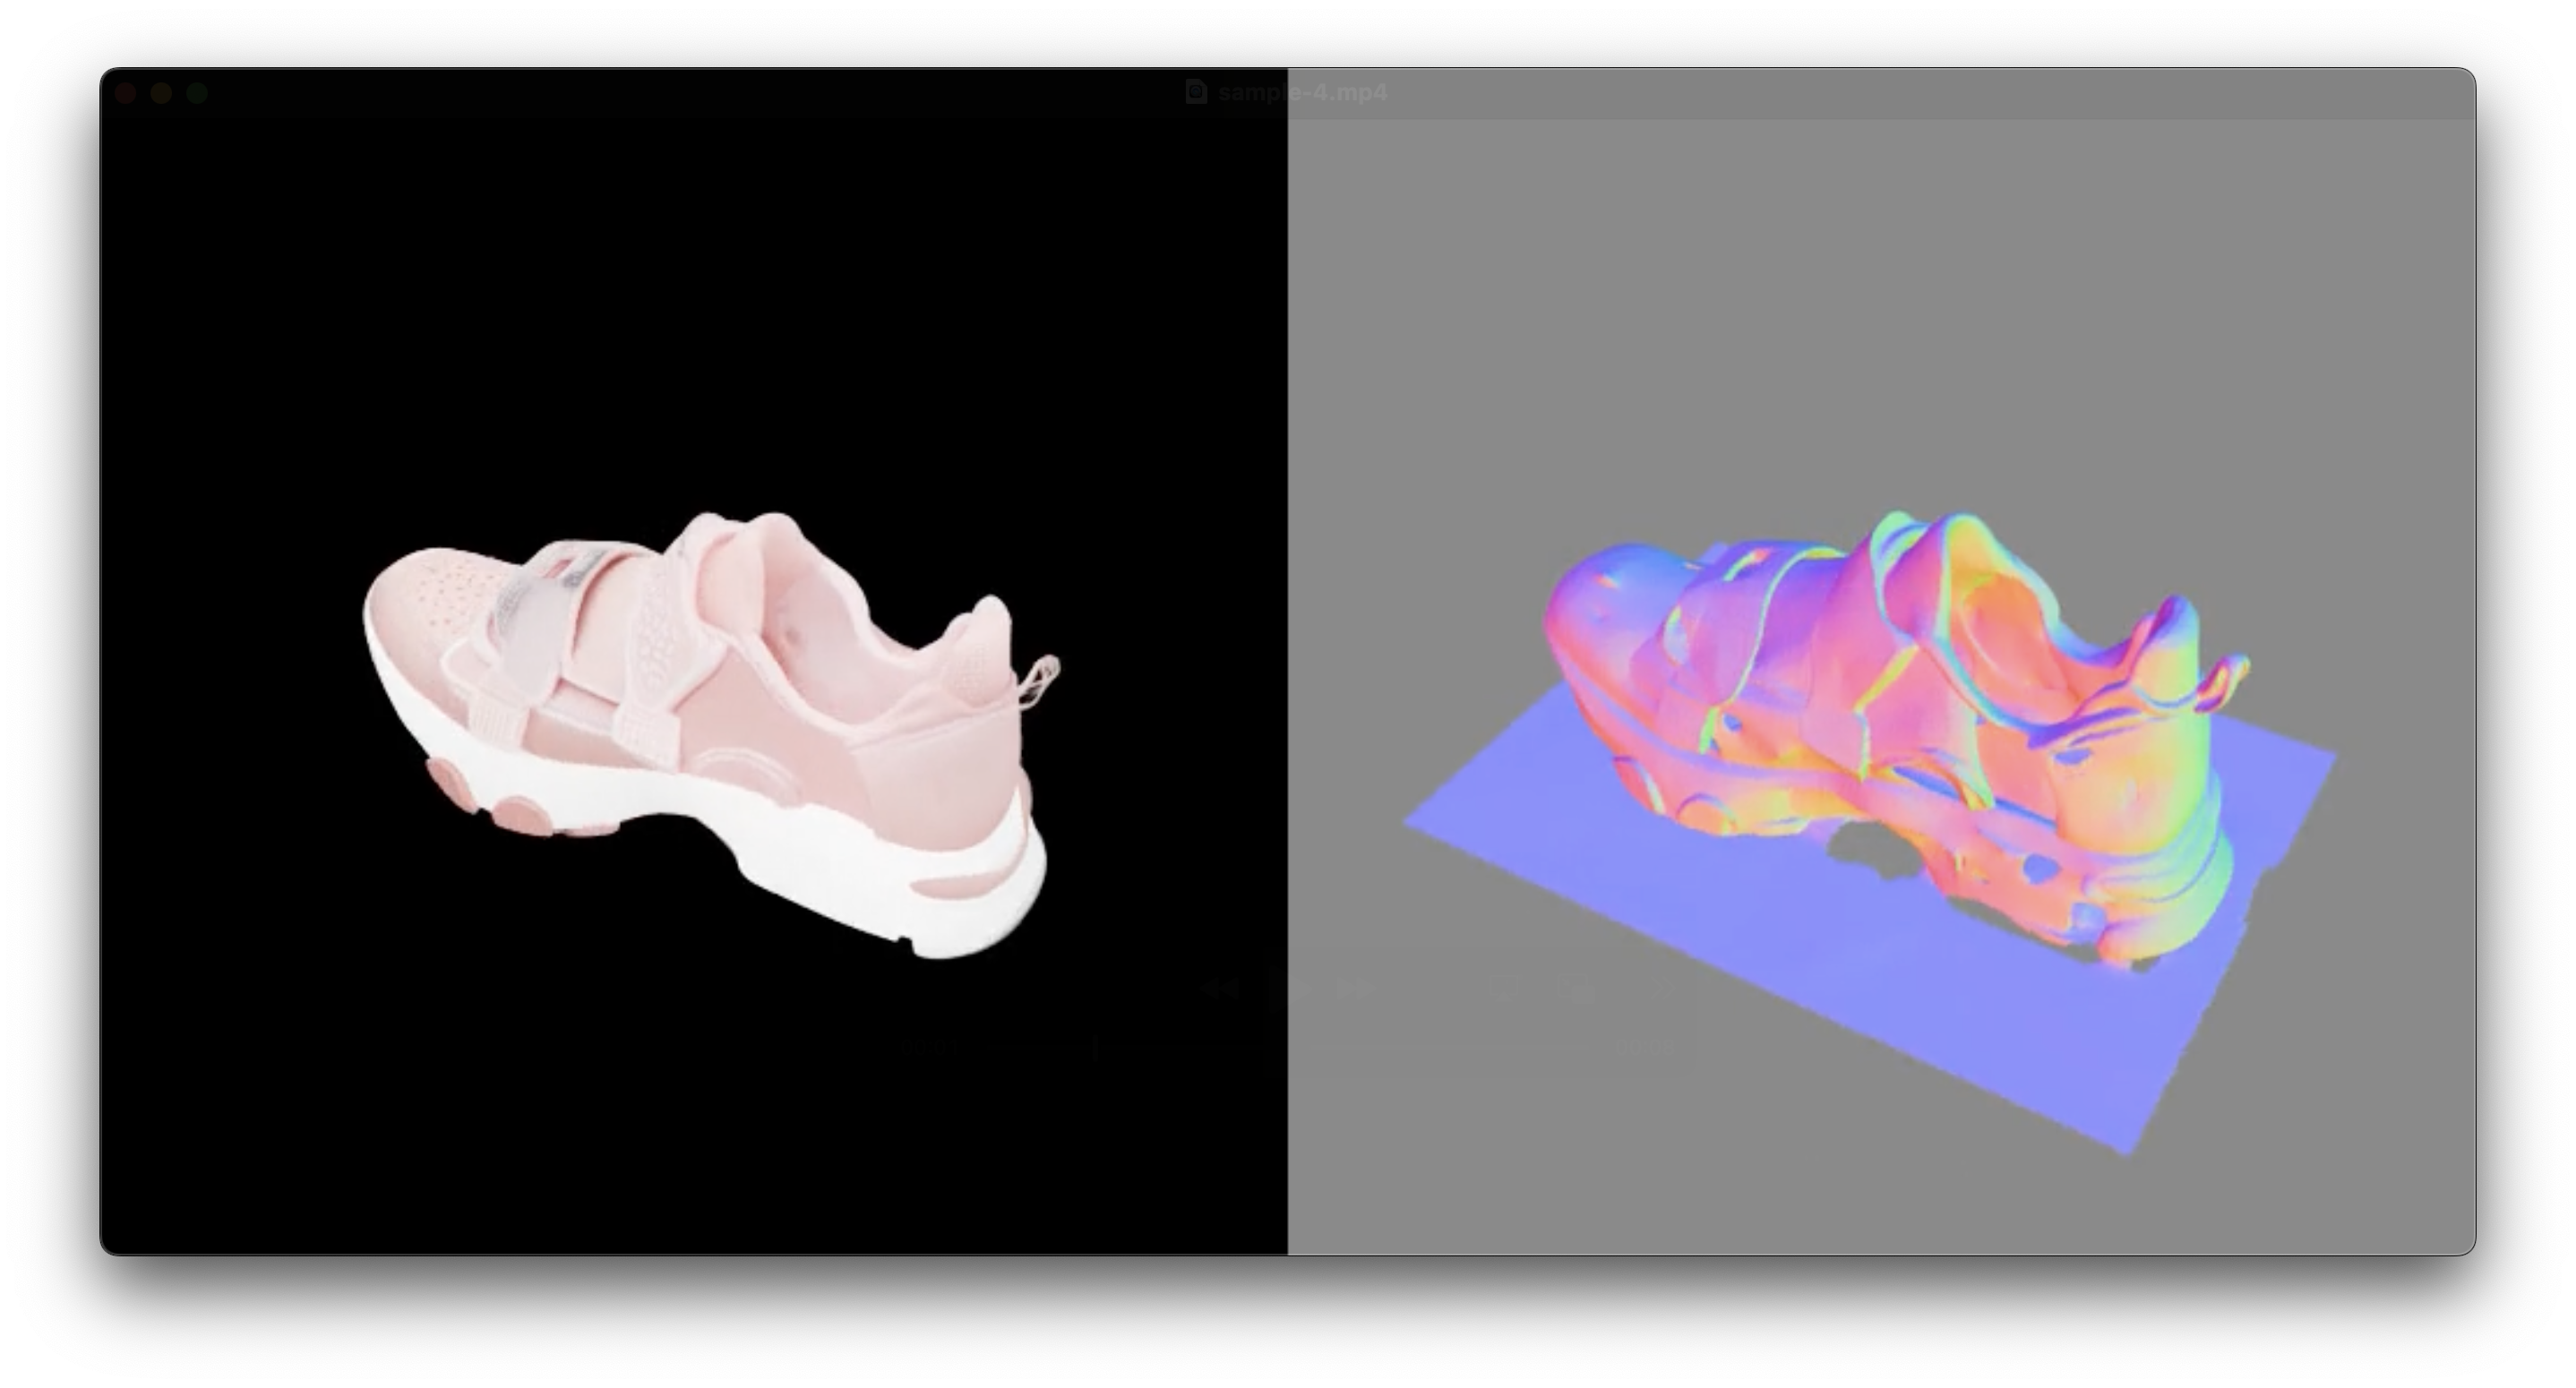
\includegraphics[width=1\textwidth]{assets/trellis_output.png}
            \caption{TRELLIS generated 3D model}
        \end{figure}
    \end{columns}
    
\end{frame}

\begin{frame}{Data augmentation avec un modèle de géneration 3D}
    % 4 images, 2x2
    \begin{figure}
        \centering
        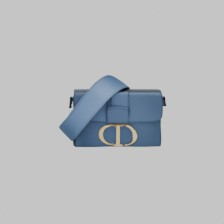
\includegraphics[width=0.35\textwidth]{assets/M9204UMOSM49E-1.jpeg}
        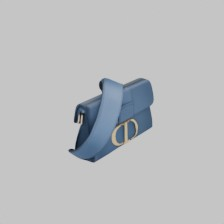
\includegraphics[width=0.35\textwidth]{assets/M9204UMOSM49E-2.jpeg}
        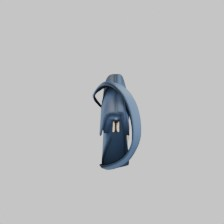
\includegraphics[width=0.35\textwidth]{assets/M9204UMOSM49E-3.jpeg}
        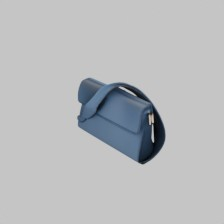
\includegraphics[width=0.35\textwidth]{assets/M9204UMOSM49E-4.jpeg}
        \caption{3D renders of a bag}
    \end{figure}
\end{frame}

\begin{frame}{Amélioration des performances grâce aux modèles 3D}
    \begin{itemize}
        \item Résultats sans l'augmentation 3D: Top-1: 36\%, Top-3: 47\%, Top-5: 59\%
        \item Nous avons d'abord ajouté les embeddings 3D à l'index.
        \item Puis nous avons retiré les embeddings 2D et avons constaté une amélioration des performances.
        \item Enfin, nous avons fusionné (moyenne des deux) les embeddings 2D et 3D pour obtenir les meilleurs résultats. Intuition: les embeddings des photos capturent des informations plus précises sur la texture, la couleur, et les embeddings 3D capturent des informations sur la forme et l'orientation.
        \item Nous avons utilisé la descente de gradients pour sélectionner les bons features ainsi que pour fusionner les embeddings 2D et 3D, mais les résultats n'était pas satisfaisants.
        \item Résultats finaux: Top-1: 45\%, Top-3: 59\%, Top-5: 64\%.
    \end{itemize}
\end{frame}

\section{User Interface}
\begin{frame}{Interface Web avec Gradio}
\begin{itemize}
    \item Interface web simple avec Gradio.
    \item Les utilisateurs peuvent uploader une photo et avoir le top-X des articles les plus similaires, ainsi que les références DAM.
\end{itemize}
\begin{figure}
    \centering
    \includegraphics[width=0.9\textwidth]{assets/gradio_interface.png}
    \caption{Interface Gradio}
\end{figure}
\end{frame}

\section{Evaluation}
\begin{frame}{Evaluation des résultats}
\begin{table}[]
    \centering
    \begin{tabular}{|c|c|c|c|}
    \hline
    \textbf{} & \textbf{Top-1} & \textbf{Top-3} & \textbf{Top-5} \\
    \hline
    Accuracy & 45\% & 59\% & 64\% \\
    \hline
    \end{tabular}
    \caption{Performances du modèle.}
\end{table}
\end{frame}

\section{Expérimentations non concluantes}
\begin{frame}{Expérimentations non concluantes}
\begin{itemize}
    \item \textbf{Tentative d'amélioration du Top-1 par NLP} :
    \begin{itemize}
        \item Utilisation du modèle BLIP Base pour générer des descriptions d'articles.
        \item Problème : Les descriptions générées sont trop pauvres pour améliorer significativement les résultats.
    \end{itemize}
\end{itemize}
\begin{table}[h]
    \centering
    \resizebox{\textwidth}{!}{%
    \begin{tabular}{c c c}
        \large \textbf{Image de test} & \large \textbf{Top-1} & \large \textbf{Top-2 (Article à trouver)} \\ 
        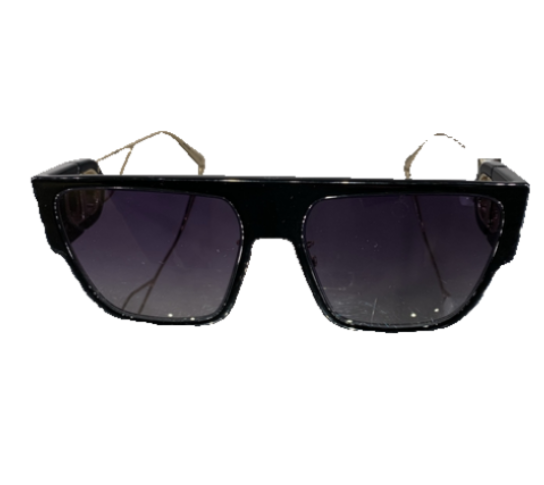
\includegraphics[width=0.5\textwidth]{assets/test_sunglasses.png} & 
        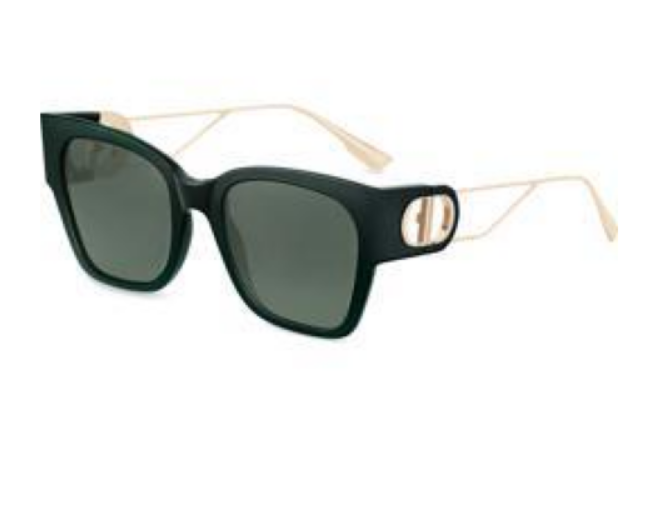
\includegraphics[width=0.5\textwidth]{assets/top1_sunglasses.png} & 
        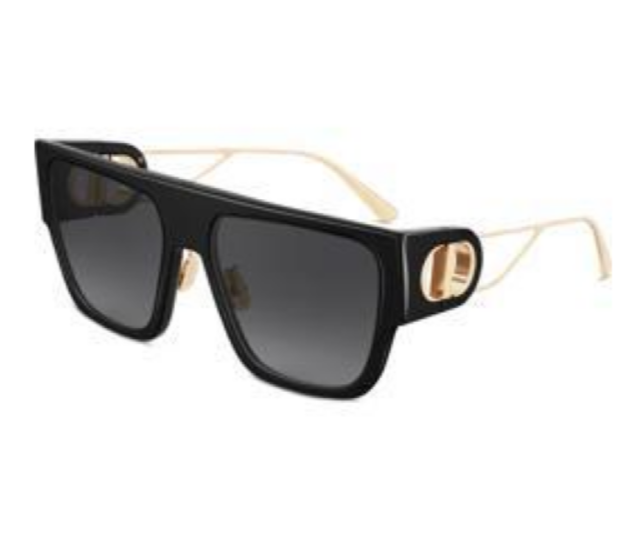
\includegraphics[width=0.5\textwidth]{assets/true_article_sunglasses.png} \\ 
        \parbox{0.3\textwidth}{\centering \large \textit{The black sunglasses with gold temples}} & 
        \parbox{0.3\textwidth}{\centering \large \textit{A pair of sunglasses with a black frame and gold arms}} & 
        \parbox{0.3\textwidth}{\centering \large \textit{A pair of sunglasses with a black frame and gold details}} \\ 
    \end{tabular}%
    }
\end{table}
\end{frame}

\begin{frame}{Expérimentations non concluantes}
\textbf{Fine-tuning de ViT :}
\begin{itemize}
        \item Faible convergence malgré un taux d'apprentissage réduit.
        \item Très long à entraîner et beaucoup de classes à prédire, pas assez de données.
\end{itemize}

\vspace{0.5cm}

\begin{figure}[h]
    \centering
    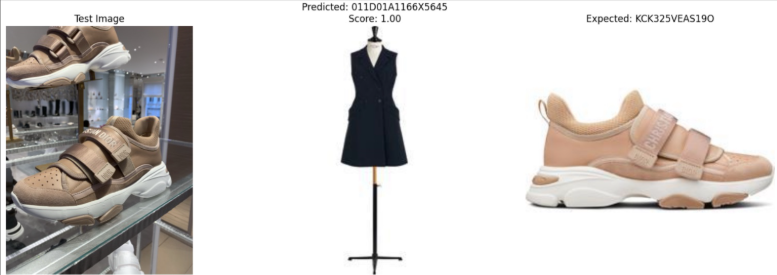
\includegraphics[width=1\textwidth]{assets/finetuning_vit.png}
    \caption{Exemple de prédiction après fine-tuning}
\end{figure}
\end{frame}

\begin{frame}{Expérimentations non concluantes}
    \begin{itemize}
            \item Siamese Network : entraîné sur la data 3D, résultats OK mais pas concluants.
            \item Réduction de dimension : PCA, AE, SAE, VAE... Meilleurs résultats avec les AE, mais pas concluants.
            \item Modèles spécialisés : FashionClip, mauvais résultats, probablement car entraîné à classifier des produits dans une catégorie générique.
    \end{itemize}

\end{frame}



\section{Conclusion}
\begin{frame}{Conclusion}
\begin{itemize}
    \item Modèle performant grâce à l'ajout de rendus 3D et la combinaison des embeddings 2D/3D.
    \item Résultats encourageants avec une précision Top-1 de 40\%, mais améliorable.
    \item Pistes futures :
    \begin{itemize}
        \item Utilisation de modèles NLP avec plus de paramètres pour enrichir les descriptions d'images et améliorer la prédiction du top-1.
    \end{itemize}
\end{itemize}
\end{frame}

\begin{frame}{Références}
    \footnotesize
    \nocite{BiRefNet}
    \bibliographystyle{plain} % Style de la bibliographie
    \bibliography{reference}  % Fichier .bib contenant les références
\end{frame}

\end{document}
